\documentclass[12pt]{article}	

\usepackage[margin=1in]{geometry}
\usepackage{amsmath,amssymb,amsthm}
\usepackage{graphicx}
\usepackage{caption}
\usepackage{subcaption}
\usepackage{url}
\usepackage{mathrsfs}
\newtheorem{theorem}{Theorem}
\newtheorem{notation}{Notation}
\newtheorem{claim}{Claim}
\newtheorem{lemma}{Lemma}
\newtheorem{definition}{Definition}
\renewcommand{\qedsymbol}{$\blacksquare$}
\newtheorem*{remark}{Remark}

\begin{document}
	\quad \quad \quad \quad \quad \quad \quad \quad \quad \quad  \quad \quad \quad \quad \quad \quad \quad \quad \quad \quad  \quad \quad \quad \quad \quad \quad \quad \quad \quad \quad  Arun Suresh
	\begin{center}
		Homework 2
	\end{center} 
	{\rule{\linewidth}{0.1mm} }
	
\indent $1. \ (a)$ The given data for $-1.5 \leq x \leq 0$ was interpolated using a linear interpolation and a cubic spline interpolation. The interpolated functions, along with the raw data was plotted against the given $x$-values, is presented below.\\
\begin{figure}[h]
	\centering
	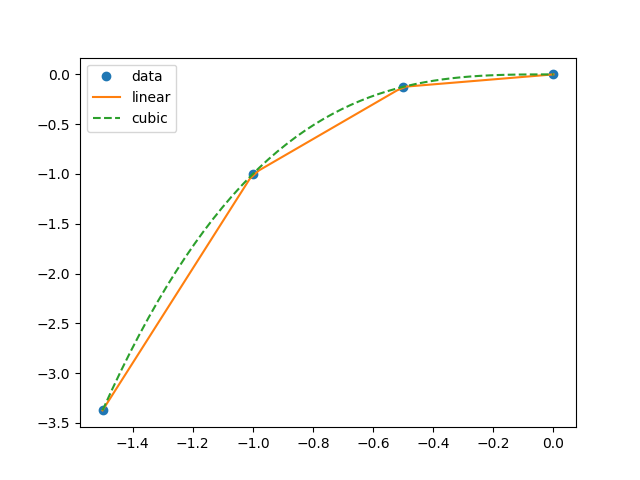
\includegraphics[scale=0.75]{1a.png}
	\caption{Linear and Cubic spline interpolation of given data}
\end{figure}
Considering that the given data depicts voltage vs. current plot for a zener-diode, we expect the cubic interpolation to the approximate data better than the linear interpolation (especially near the breakdown-voltage)
\newpage
\indent $1. \ (b)$ More sample points were added to the data and the full data set ($-1.5 \leq x \leq 4.5$) was interpolated once again using a linear and a cubic spline. The interpolated functions, along with the raw data was plotted against the given $x$-values, is prestented below.\\\\
	\begin{figure}[h]
		\centering
		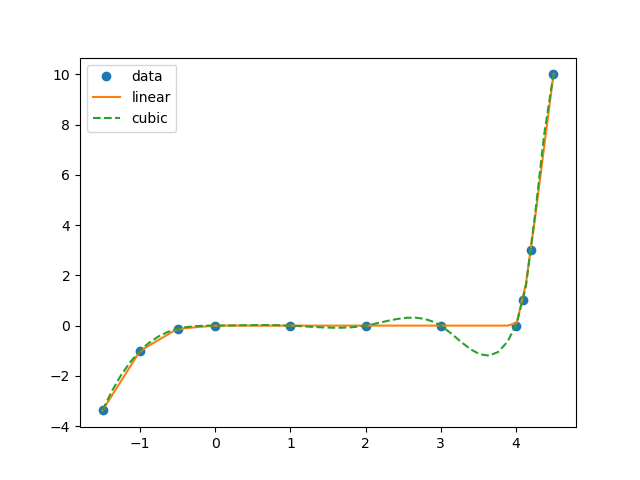
\includegraphics[scale=0.75]{1b.png}
		\caption{Linear and Cubic spline interpolation of given data}
	\end{figure}\\\\
Once again, we expect the cubic interpolation to predict the data better than a linear interpolation, at least near the breakdown regions. \\\\ However, since the breakdown region (around $3.8 - 4.0$) is very sensitive to small changes in $x$, more data is needed there to produce a satisfactory cubic interpolation.
Lack of data around the specified region is the reason we observe a comparitively significant deviation (from the expected zener I-V characteristic curve) in the cubic interpolating function near $x = 3.8$.
\newpage
\indent $1. \ (c)$ The function $f(x) = \sin(x)$ was interpolated using function values at various arguments equally spaced between $0$ and $2\pi$. Three different spline interpolations were produced to test the effectiveness of higher order interpolation methods. The interpolated functions, along with the actual $\sin(x)$ function, are plotted against the given $x$ values. Adding more data points helped improve the accuracy of the interpolations. Plots with $5$, $6$ and $10$ data points were generated, and the results are presented below.

\begin{figure}[h]
	\begin{subfigure}[h]{0.3\textwidth}
		\centering
		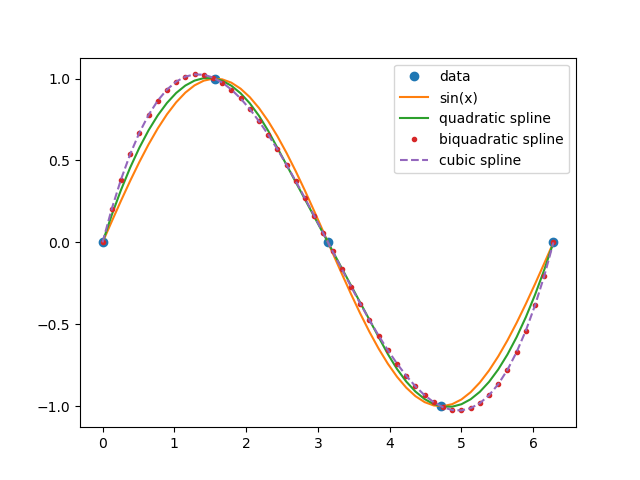
\includegraphics[width=\textwidth]{1cn5.png}
		\caption{$5$ data points}
	\end{subfigure}
	\hfill
	\begin{subfigure}[h]{0.3\textwidth}
		\centering
		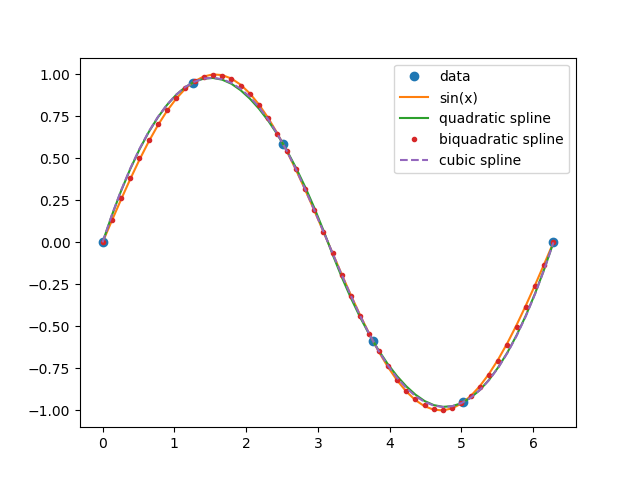
\includegraphics[width=\textwidth]{1cn6.png}
		\caption{$6$ data points}
	\end{subfigure}
	\hfill
	\begin{subfigure}[h]{0.3\textwidth}
		\centering
		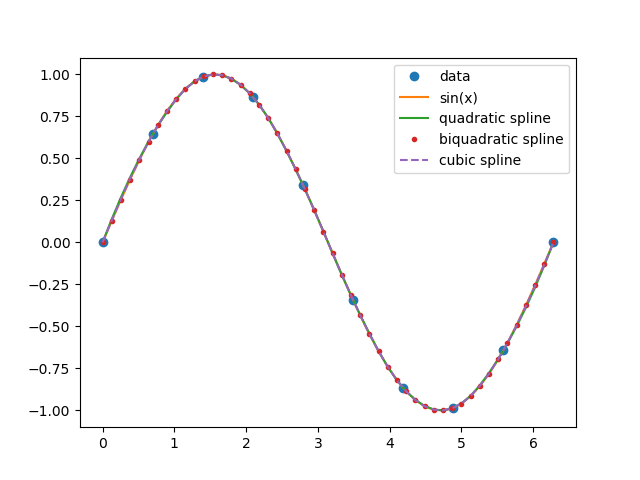
\includegraphics[width=\textwidth]{1cn10.png}
		\caption{$10$ data points}
	\end{subfigure}
	\caption{Interpolated functions}
\end{figure}

Higher order (cubic and biquadratic) interpolations were able to approximate the function to a much better degree, as more data points were added - however, with a lesser number of data points, the lower order quadratic interpolation was able to approximate the function better. \\\\ A section of the plot, zoomed close to the region near the local maxima (where the second derivative is maximum), is presented below for $6$ and $10$ data points, which allows us to see the degree of effectiveness of the higher order interpolations. The plots were magnified until the differences between interpolation and the original function was observed. 
\begin{figure}[h]
	\begin{subfigure}[h]{0.5\textwidth}
		\centering
		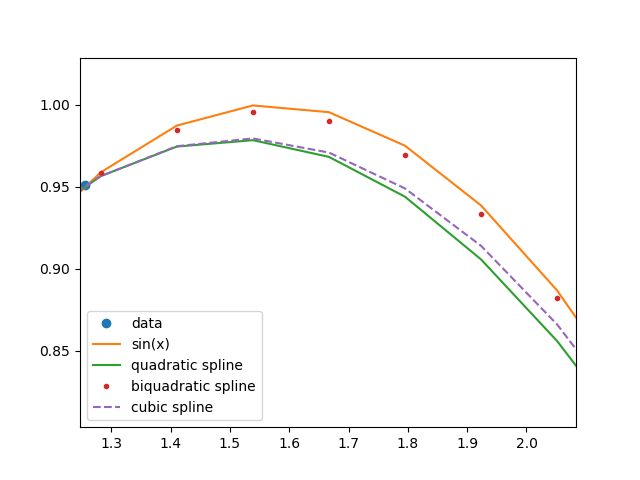
\includegraphics[width=\textwidth]{1cn6zoom.png}
		\caption{$6$ data points}
	\end{subfigure}
	\hfill
	\begin{subfigure}[h]{0.5\textwidth}
		\centering
		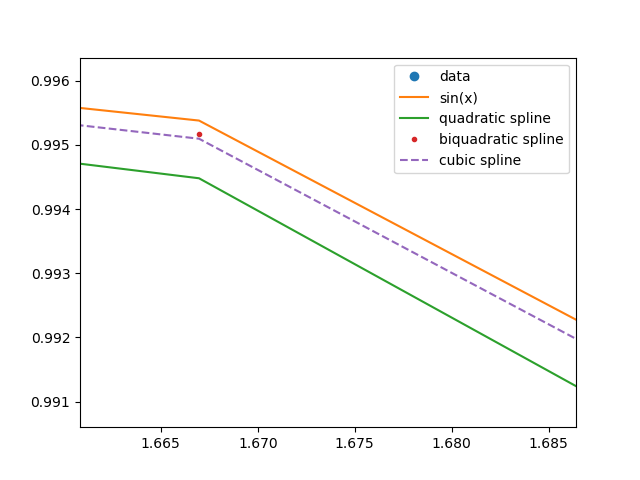
\includegraphics[width=\textwidth]{1cn10zoom.png}
		\caption{$10$ data points}
	\end{subfigure}
	\caption{Interpolated functions - zoomed to maxima}
\end{figure}
\newpage
\indent $1. \ (d)$ The oscillatory behavior of the step and pulse function was studied and interpolated against the given arguements. The interpolation was done using the zeroth order spline for both of the given functions. This type of interpolation was chosen because of the discrete nature of the given functions, and the abrupt discontinuities present in the data. Since at any point away from the neighborhood around zero, both functions took on constant values, the most natural interpolation to choose was that which used constant functions (zero-th order interpolation). The interpolated functions, along with the data points for both the pulse and step functions are plotted below. 
\begin{figure}[h]
	\centering
	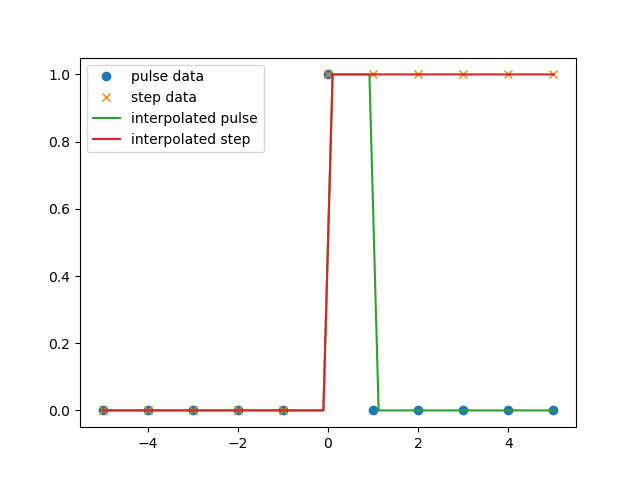
\includegraphics[scale=0.75]{1d.png}
	\caption{Interpolation of pulse and step functions}
\end{figure}

\newpage
2. The given data was interpolated using three different interpolating functions. These were - Lagrange interpolation, zero-th order interpolation and "nearest snap" interpolation. \\

\textbf{Note:} The nearest snap interpolation is provided by the scipy package for python, and is not a traditional interpolation method. However, it is very good in interpolating discrete functions with abdrupt discontinuities in them. The interpolation technique obtains the data, records the nearest $x$ value as its argument, and makes the interpolating function take the $y$ value corresponding to its current argument. This $y$ value in the interpolating function is held constant as the compiler slowly increments $x$ by some predefined step-size. When it finds another $x$ value in the given data that is closer, the interpolating function snaps to having the $y$ value corresponding to this newly obtained $x$ value. This process repeats until all the input data values have been extinguished.  \\ \indent It is easy to notice that this nearest snap interpolation is very close to a zero-th order spline interpolation - except, the interpolating function is artifically constructed to model the discrete nature of the given data. The data is assumed to be the difference of two step-functions. \\\\


The error corresponding to each interpolation was calculated by defining the given data as a function (increasing the resolution of the given data by adding 50 other data points). The interpolated functions were then subtracted from this extended function to study the error present in each one of them. It is easy to observe that the error given by zero-th order spline and the nearest snap, are comparable. However, in comparison to these two, the lagrange interpolation (which was cubic) did very poorly in interpolating the data. All of the error can be attributed to the abdrupt discontinuities in the given data. The interpolated functions along with the given data points, and the error plots are plotted below \\

\begin{figure}[h]
	\begin{subfigure}[h]{0.5\textwidth}
		\centering
		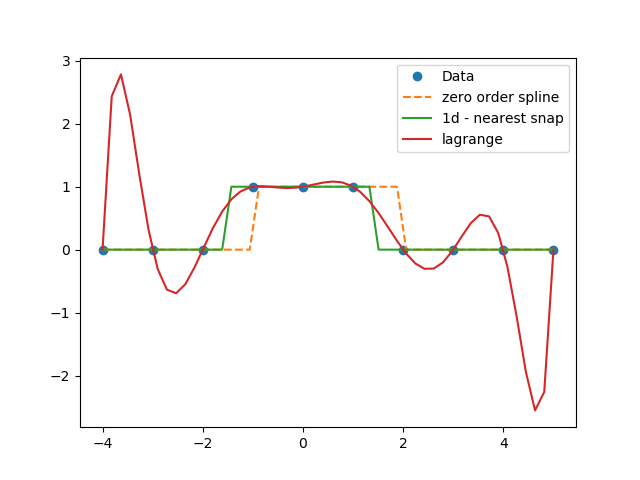
\includegraphics[width=\textwidth]{2plot.png}
		\caption{plot}
	\end{subfigure}
	\hfill
	\begin{subfigure}[h]{0.5\textwidth}
		\centering
		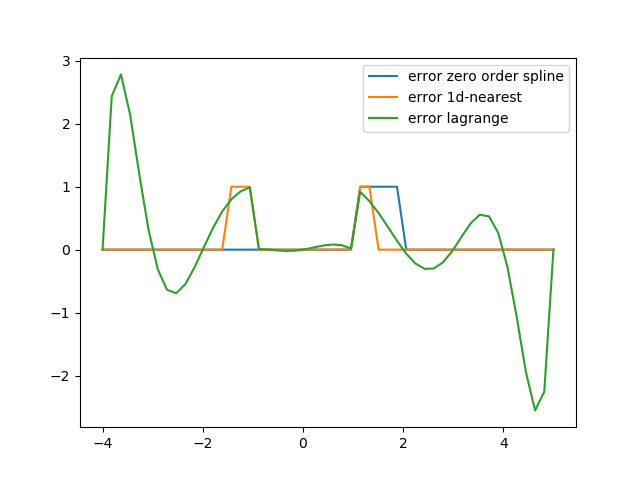
\includegraphics[width=\textwidth]{2error.png}
		\caption{error}
	\end{subfigure}
	\caption{Three different interpolation functions approximating the given data}
\end{figure}
\end{document}